\section{Discussion and Conclusion}\label{sec:conclusion}

We have measured the local PNG parameter $\fnl$ using the scale-dependent bias in the angular clustering of LRGs selected from the DESI Legacy Imaging Survey DR9. Our sample includes more than $12$ million LRG targets covering around $14,000$ square degrees in the redshift range of $0.2< z < 1.35$. We leverage early spectroscopy during DESI Survey Validation \citep{desi2023sv} to infer the redshift distribution of our sample (Figure \ref{fig:nz}). \mr{Our power spectrum model accounts for various theoretical and observational effects such as RSD, magnification bias, survey geometry, and integral constraint. Most importantly, we utilize a novel machine learning-method to mitigate the effect of imaging systematics and reduce excess clustering power at low $\ell$.}

In our fiducial analysis, \mr{which includes non-linear treatment using nine maps (Galactic extinction, stellar density, depth in $grzW1$, and psfsize in $grz$), we obtain $\fnl = 34^{+24(+50)}_{-44(-73)}$ with $p=1$ and $s=0.945$, which is consistent with recent CMB and LSS measurements, as visualized in Figure \ref{fig:fnlhist}. Our constraints are robust against $p$ and $s$ (Figure \ref{fig:fnl_magbias}). The signature of local PNG is very sensitive to excess clustering power caused by imaging systematic effects. We have applied a series of robustness tests to investigate the impact of how the galaxy selection function is determined. Specifically, both linear and nonlinear methods are applied using various combinations of imaging systematic maps (including two external maps for the neutral hydrogen column density and photometric calibration error in the z band). We also examine the effect of additional masks based on imaging properties and survey completeness. Overall, we find no change in the analysis that shifts the maximum likelihood value of $\fnl$ to a significantly different value (Figure \ref{fig:mcmc_dr9reg}, Figure \ref{fig:mcmc_dr9elmin}, and Table \ref{tab:dr9method}).}

\begin{figure}
    \centering
    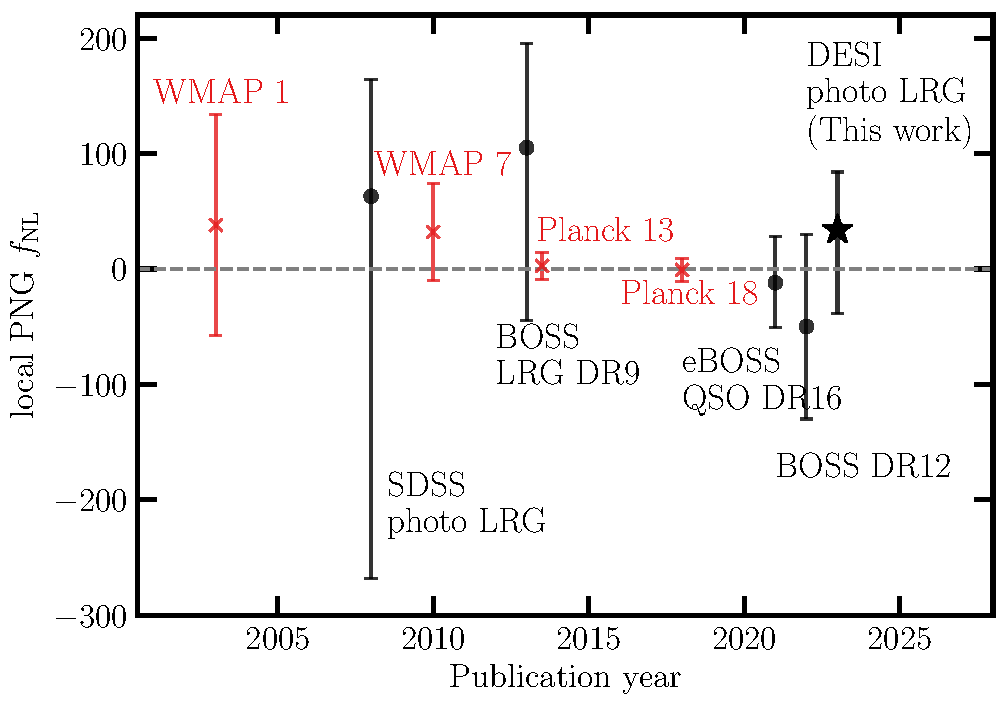
\includegraphics[width=0.45\textwidth]{figures/fnl_history.pdf}
    \caption{History of constraints on local PNG $\fnl$ at $95\%$ confidence from single-tracer LSS \citep{slosar2008constraints,2013MNRAS.428.1116R, mueller2022primordial, 2022PhRvD.106d3506C}, including our analysis with $\mr{-39}<\fnl<\mr{84}$ (DESI photo LRG) and CMB surveys \citep{Komatsu_2003, Komatsu_2010, planck13, akrami2019planck}. The median $\fnl$ value is used in case the maximum likelihood estimate was not reported in the reference.}
    \label{fig:fnlhist}
\end{figure}

\mr{It is imperative to stress that the template-based approach, which is applied to the dataset to address large-scale excess clustering caused by imaging systematics, inevitably removes large-scale clustering information. Mitigating with more maps removes more of the power spectrum and biases the $\fnl$ posterior distribution. We can de-bias the constraints to increase the accuracy of our results, however the process degrades the precision on $\fnl$. We try regressions of systematics using a smaller set of maps as an attempt to avoid over-fitting the large-scale clustering signal. We utilize the mean galaxy density and cross correlations of the galaxy density field and imaging property maps to identify the least number of maps (Appendix \ref{sec:systests}).  Unfortunately, these tests depend on the $\fnl$ value used in the mocks, and therefore they reveal a preference for artificially diminishing the constraining power of the dataset, as we consistently remove excess clustering signal until $\fnl=0$ is recovered (for instance, if we consider the covariances constrcuted from the $\fnl=0$ mocks). While we can recover the removed signal and debias the $\fnl$ posterior after accounting for over-correction, we lose constraining power due to the removal of large-scale clustering information. Hence, there is a strong motivation for exploring alternative approaches that avoid over-correction and enhance the science yield of datasets in future studies of local primordial non-Gaussianity.}

\mr{Galactic extinction, depth in z, and psfsize in r are identified as the primary sources of systematics. The non-linear method with three maps is able to mitigate most of the trends against all available templates, but it yields an $\fnl$ result that is highly degenerate with unforeseen excess power on large scales. In spite of the fact that the nonlinear three maps does not pass our validation tests, however, we find that the constraining power is almost twice stronger than that of the nonlinear nine maps. This results motivates that finding an optimal set of imaging property maps can avoid erasing large-scale clustering information and enhanace the precision of the analysis.} Our analysis can be considered as the first attempt to identify major systematics in DESI, so we can be ready for constraining $\fnl$ with DESI spectroscopy. Internal DESI tests of the photometric calibration were unable to uncover DESI-specific issues, e.g., when comparing to Gaia data. The most significant trends that we find are with the E(B-V) map. The source of such a trend would be a mis-calibration of the E(B-V) map itself or the coefficients applied to obtain Galactic extinction corrected photometry. Such a mis-calibration would plausibly be proportional in amplitude to the estimated E(B-V) map, though it may not have E(B-V)’s spatial distribution. In order to explain the $\fnl$ signal we measure using nonlinear three maps, such an effect would need to be approximately twice that of the trend we find with E(B-V). There are ongoing efforts within DESI to obtain improved Galactic extinction information, which will help establish if this is indeed the cause. \mr{Additionally, cross-correlations of the DESI LRG density with the CMB lensing map is more stable in terms of systematics and can complement analyses based on galaxy-galaxy clustering. We can further improve the estimation of the galaxy survey selection function by combining our neural network-based method with forward-modeling techniques, such as Obiwon \citep{kong2020}, but we will leave that for future work.} 
